\section{Feynman diagrams}\label{sec:4.8}

An electron injected \SI{5}{eV} above the conduction-band edge of silicon does not stay there for long. It knocks electrons across the gap and emits phonons, and its quasiparticle peak acquires the width $\varGamma_{\mathrm{qp}} = -2z_{\mathrm{qp}}\Imag\Sigma^{\mathrm{R}}$ of \cref{eq:4.7-qp}. To get a number we need $\Sigma$, and the self-energy of an interacting system can only be computed as a series in the interaction. The same is true of the density response beyond the independent-electron bubble of \cref{sec:4.5}. Feynman diagrams are the bookkeeping for these series: each term of the expansion is a picture, and a small set of rules turns the picture into an integral. The treatment follows Refs.~\cite{bruus2004many}, \cite[Chaps.~3 and 7]{fetter1971quantum} and \cite[Chaps.~2 and 3]{mahan2000many}.

\subsection{Wick's theorem and the rules}

Split $H_\mu = H_0 + H_{\mathrm{int}}$, with $H_0 = \sum_{\vect{k}}\xi_{\vect{k}}c^\dagger_{\vect{k}}c_{\vect{k}}$ the independent electrons of \cref{sec:4.7}. In imaginary time the Boltzmann factor and the Heisenberg operators can both be written with the ordered exponential $U_{\mathrm{I}}(\beta,0) = \mathrm{T}_\tau\exp[-\int_0^\beta\dd\tau\,H_{\mathrm{int},\mathrm{I}}(\tau)]$, where the subscript I marks operators that evolve with $H_0$ alone. The Matsubara Green's function \cref{eq:4.7-Gtau} becomes the ratio \cref{eq:D.11-Gexp},
\begin{equation*}
  \GF(\vect{k},\tau) = -\frac{\bigl\langle\mathrm{T}_\tau\,U_{\mathrm{I}}(\beta,0)\,c_{\vect{k},\mathrm{I}}(\tau)\,c^\dagger_{\vect{k},\mathrm{I}}(0)\bigr\rangle_0}{\bigl\langle U_{\mathrm{I}}(\beta,0)\bigr\rangle_0} ,
\end{equation*}
with $\langle\cdots\rangle_0$ the average in the free grand-canonical state. Expanding the exponential, the term of order $n$ in $H_{\mathrm{int}}$ is an integral over $n$ imaginary times of a free average of a time-ordered string of creation and annihilation operators. Nothing has been approximated so far.

Wick's theorem evaluates these averages~\cite{wick1950evaluation}. In the free state, the time-ordered average of a string of fermion operators is a sum over all ways of grouping the operators into pairs. Each grouping contributes the product of its pair averages, with the sign of the permutation that brings the members of every pair next to each other. Only pairs of one creation and one annihilation operator of the same mode survive. Their time-ordered averages, the contractions, are free Green's functions:
\begin{equation}
  \bigl\langle\mathrm{T}_\tau\,c_{\vect{k},\mathrm{I}}(\tau)\,c^\dagger_{\vect{k},\mathrm{I}}(\tau')\bigr\rangle_0 = -\GF_0(\vect{k},\tau - \tau') .
  \label{eq:4.8-contract}
\end{equation}
For bosons the same holds without signs, and a contraction of the field $d_{\vect{Q}} + d^\dagger_{-\vect{Q}}$ with itself is the free boson propagator. The theorem is the quantum version of the statement that every moment of a Gaussian distribution is a sum over pairings (\cref{app:C.6}): the free grand-canonical state is the ``Gaussian'' state of the many-body problem. \Cref{app:D.11} proves it with Gaudin's trace argument~\cite{gaudin1960demonstration}, which uses only the anticommutators and the cyclic property of the trace. At $T = 0$ the same theorem holds for averages in the Fermi sea $|\Phi_0\rangle$, the limit $\beta \to \infty$ of the free state, with the contraction $\ii\GF_0(\vect{k},t - t')$ of the time-ordered function \cref{eq:4.7-GT}. The interacting ground state is reached from $|\Phi_0\rangle$ by switching on the interaction slowly, as long as no level crossing intervenes (the theorem of Gell-Mann and Low~\cite{gellmann1951bound}), and the real-time expansion \cref{eq:D.11-GT} has the same structure.

Each pairing is drawn as a picture. A contraction \cref{eq:4.8-contract} is a solid line with an arrow, from the point where the electron is created to the point where it is annihilated. A factor $H_{\mathrm{int}}$ is a vertex, or for the Coulomb interaction a dashed line whose two ends are the two density operators of the pair interaction. Pairings that fall into a piece attached to the external points and a piece that is not, the vacuum diagrams, cancel against the denominator, which is the linked-cluster theorem, and only connected diagrams remain. Relabeling the $n$ identical interaction factors, and exchanging the two ends of each line, produces $n!\,2^n$ pairings with the same value, which cancel the $1/n!$ of the exponential and the $\tfrac12$ of the pair interaction. Collecting the signs and the factors of $T$ and $\Vol$, \cref{app:D.11} arrives at the following rules.
\begin{keyresult}[Feynman rules in imaginary time]
The Green's function $\GF(\vect{k},\ii\omega^{\mathrm{F}}_j)$ is the sum of all connected, topologically distinct diagrams with two external points, each evaluated with the following factors.
\begin{enumerate}
  \item Each solid line carrying $(\vect{p},\ii\omega^{\mathrm{F}})$ is $\GF_0(\vect{p},\ii\omega^{\mathrm{F}}) = 1/(\ii\omega^{\mathrm{F}} - \xi_{\vect{p}})$; spin is conserved along it.
  \item Each Coulomb line carrying $(\vect{k},\ii\omega^{\mathrm{B}})$ is $-v_{\mathrm{C}}(k)/\Vol$. Each boson line is $-|g(\vect{Q})|^2\mathsf{D}_0(\vect{Q},\ii\omega^{\mathrm{B}})/\Vol$, with $\mathsf{D}_0(\vect{Q},\ii\omega^{\mathrm{B}}) = 2\omega_{\vect{Q}}/[(\ii\omega^{\mathrm{B}})^2 - \omega_{\vect{Q}}^2]$ for a boson of energy $\omega_{\vect{Q}}$ coupled through $H_{\mathrm{int}} = \Vol^{-1/2}\sum g(\vect{Q})\,c^\dagger_{\vect{k}+\vect{Q}}c_{\vect{k}}(d_{\vect{Q}} + d^\dagger_{-\vect{Q}})$.
  \item Momentum and frequency are conserved at every vertex. Each independent internal momentum is summed, and each independent internal frequency carries $T\sum_j$.
  \item Each closed fermion loop gives $-1$ and a sum over its spin.
  \item A solid line that begins and ends on the same interaction carries $\ee^{\ii\omega^{\mathrm{F}}0^+}$.
\end{enumerate}
The response function \cref{eq:4.7-Rtau} of two densities is $-1/\Vol$ times the sum of connected diagrams with two density vertices, at which $\vect{q}$ and $\ii\omega^{\mathrm{B}}_j$ enter and leave, evaluated with the same rules. At $T = 0$ the rules for the time-ordered functions are the same with $\GF_0(\vect{p},\omega) = 1/(\omega - \xi_{\vect{p}} + \ii0^+\operatorname{sgn}\xi_{\vect{p}})$, each Coulomb line $+\ii v_{\mathrm{C}}(k)/\Vol$, and each internal frequency $\int\dd\omega/2\pi$, and the time-ordered response $-(\ii/\Vol)\langle\mathrm{T}\,O_a(\vect{q},t)^\dagger O_b(\vect{q},0)\rangle$ carries $+\ii/\Vol$ in place of $-1/\Vol$.
\end{keyresult}
The sign of a loop is the one rule that has no counterpart in the old-fashioned perturbation theory of \cref{sec:2.4}. It comes from the last contraction around the loop, which pairs the first creation operator with the last annihilation operator and costs an odd number of exchanges. The rule for the response function needs one line of its own. The definition \cref{eq:4.7-Rtau} carries $-1/\Vol$. A response diagram has $2n + 2$ propagators at order $n$, an even number, so the $-1$ of each contraction drops out. The signs left over are those of the expansion, $(-1)^n$, which the rule puts into the lines, and of the loops. \Cref{app:D.11} checks the rules for $\GF$ at first order against the Hartree--Fock self-energy. The next subsection checks the rule for $R$ against \cref{eq:4.7-bubble} and against the screening of \cref{sec:4.4}.

In the frequency representation every line is a simple pole, every frequency sum is done by the residue formula \cref{eq:C.5-matsum}, and the temperature enters only through these sums: $\GF_0$ and $\mathsf{D}_0$ do not depend on it, and the occupation factors $n_{\mathrm{F}}$ and $n_{\mathrm{B}}$ appear as residues of $n_{\mathrm{F}}(z)$ and $n_{\mathrm{B}}(z)$.

\subsection{The bubble and the random-phase chain}

The density response of independent electrons is the simplest diagram there is: one fermion loop through the two density vertices (\cref{fig:4-diagrams}a). An electron is created in $\vect{k} + \vect{q}$ and a hole in $\vect{k}$ at one vertex, and both are annihilated at the other. By the rules, the loop contributes $-1$ and a spin sum, the two lines give $\GF_0(\vect{k},\ii\omega^{\mathrm{F}}_{j'})\GF_0(\vect{k}+\vect{q},\ii\omega^{\mathrm{F}}_{j'} + \ii\omega^{\mathrm{B}}_j)$, and the internal momentum and frequency are summed. With the $-1/\Vol$ of the response,
\begin{equation}
  R^0(\vect{q},\ii\omega^{\mathrm{B}}_j) = \frac1\Vol\sum_{\vect{k}s}T\sum_{j'}\GF_0(\vect{k},\ii\omega^{\mathrm{F}}_{j'})\,\GF_0(\vect{k}+\vect{q},\ii\omega^{\mathrm{F}}_{j'} + \ii\omega^{\mathrm{B}}_j) ,
  \label{eq:4.8-bubble}
\end{equation}
which is the first form of \cref{eq:4.7-bubble}. The frequency sum is \cref{eq:D.10-sum}, and it produces the Pauli difference $[n_{\mathrm{F}}(\xi_{\vect{k}}) - n_{\mathrm{F}}(\xi_{\vect{k}+\vect{q}})]/(\ii\omega^{\mathrm{B}}_j + \xi_{\vect{k}} - \xi_{\vect{k}+\vect{q}})$. Continued to $\omega + \ii0^+$ by \cref{eq:4.7-Rcont}, this is the independent-electron response \cref{eq:4.5-R0}, whose evaluation for the electron gas is the Lindhard function of \cref{sec:4.5}. In a crystal the plane waves become Bloch states $\psi_{n\vect{k}}$, the density vertex $n_e(\vect{q}+\vect{G})$ acquires the matrix element $\rho_{mn}(\vect{k},\vect{q}+\vect{G})$ between the two states it connects, and the same diagram is the crystal bubble \cref{eq:4.6-R0} (\cref{eq:D.12-R,eq:D.12-L0}). The sign of the rule passes its first test: the static bubble is negative, as a response must be.

\begin{figure}[tbp]
  \centering
  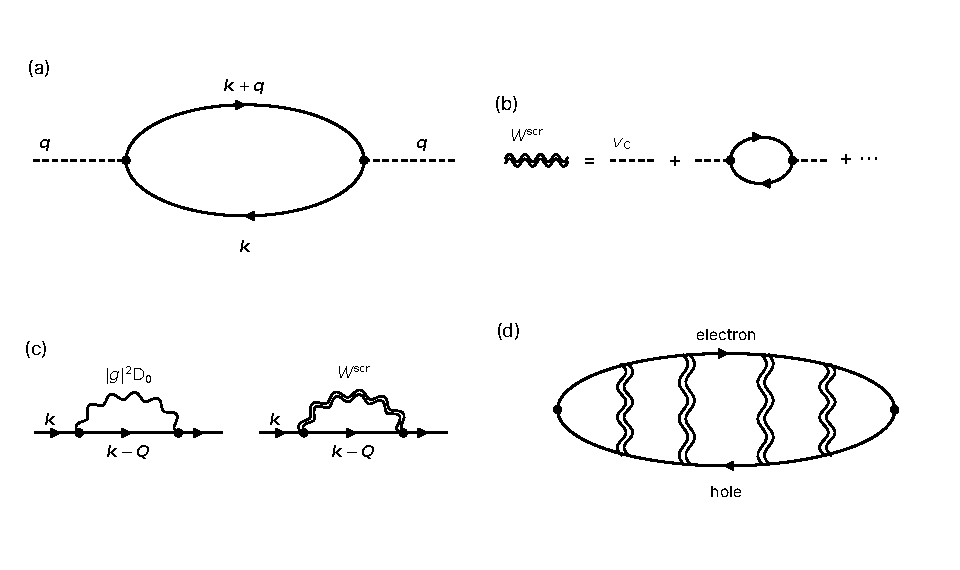
\includegraphics[width=\linewidth]{figures/ch04/fig4_9.pdf}
  \caption{The diagrams of \cref{sec:4.8}. Solid lines with arrows are free electron propagators $\GF_0$; an arrow against the direction of the momentum label is a hole. Dashed lines are the bare Coulomb interaction $v_{\mathrm{C}}$, except the short dashed stubs in (a), which mark the external momentum $\vect{q}$ entering and leaving at the density vertices; single wavy lines a boson, double wavy lines the screened interaction $W^{\mathrm{scr}}$. Dots are vertices. (a) The bubble: a density vertex creates an electron in $\vect{k}+\vect{q}$ and a hole in $\vect{k}$, and a second vertex annihilates them; it is the independent-electron response $R^0$. (b) The screened interaction as the random-phase chain of bubbles joined by Coulomb lines, $W^{\mathrm{scr}} = v_{\mathrm{C}} + v_{\mathrm{C}}R^0v_{\mathrm{C}} + \cdots$. (c) The self-energy of an electron that emits and reabsorbs a boson, with the line $|g|^2\mathsf{D}_0$, and the $GW$ self-energy, the same diagram with the screened line. (d) The ladder: the electron and the hole of the bubble interact through screened interaction lines. Summed together with the chain of exchange lines, it becomes the Bethe--Salpeter equation of \cref{sec:4.9}.}
  \label{fig:4-diagrams}
\end{figure}

At first order in $v_{\mathrm{C}}$ the bubble is corrected by three kinds of diagram, which differ in where the Coulomb line attaches. It can join two bubbles, the line carrying the momentum $\vect{q}$ from one to the other. It can run across the bubble, from the electron line to the hole line. Or it can begin and end on one propagator, which is a first-order self-energy inserted into that line. The first kind has two loops, and by the rules its value is $-(1/\Vol)(-1)^2(-v_{\mathrm{C}}(q)/\Vol)\,(\Vol R^0)(\Vol R^0) = R^0v_{\mathrm{C}}(q)R^0$, with a plus sign, where each loop without its sign is $\sum_{\vect{k}s}T\sum_{j'}\GF_0\GF_0 = \Vol R^0$. The second kind has the same propagators and the same line but only one loop, and the opposite sign. Repeating the first kind gives the chain $R^0 + R^0v_{\mathrm{C}}R^0 + R^0v_{\mathrm{C}}R^0v_{\mathrm{C}}R^0 + \cdots$, a geometric series with the sum
\begin{equation}
  R = \frac{R^0}{1 - v_{\mathrm{C}}(q)R^0} .
  \label{eq:4.8-chain}
\end{equation}
This is the random-phase approximation \cref{eq:4.5-rpa}, now as a definite selection of diagrams: the chain of bubbles, and nothing inside them. Its sign is the one \cref{sec:4.4} found from the classical argument, $\varepsilon = 1 - v_{\mathrm{C}}R^0 > 1$ in the static limit. The general statement is just as direct. A diagram for $R$ either can or cannot be cut into two by cutting a single Coulomb line at the momentum $\vect{q}$. Call the sum of those that cannot the proper part $\tilde R$. Every diagram that can is a chain of proper pieces joined by such lines, and the sum of the chains is $R = \tilde R + \tilde Rv_{\mathrm{C}}R$, the Dyson equation \cref{eq:4.4-dyson}. The blobs of \cref{fig:4-series} are sums of Feynman diagrams, and the random-phase approximation keeps the bubble alone in each blob.

In a crystal the Coulomb line between two bubbles carries $\vect{q} + \vect{G}$ for every reciprocal-lattice vector $\vect{G}$, and the chain becomes the matrix equation of \cref{sec:4.6}. The line with $\vect{G} = 0$ carries the macroscopic field. The lines with $\vect{G} \ne 0$ are the local fields, and in the language of transitions they form the exchange kernel $K^{\mathrm{x}}$ of \cref{sec:4.6}, the Coulomb interaction without its $\vect{G} = 0$ term. The second kind of first-order diagram, the line across the bubble, is the attraction between the electron and the hole that the chain leaves out. Repeated, with each interaction line screened by its own chain of bubbles, it forms the ladder of \cref{fig:4-diagrams}d. The sum of ladders and exchange chains is the Bethe--Salpeter equation, the equation for an electron--hole pair that propagates while the two particles attract each other, and its bound states are the excitons of \cref{sec:4.9}. \Cref{app:D.12} derives it from these diagrams, with the direct kernel $K^{\mathrm{d}}$ built from the screened interaction line.

\subsection{Reducible lines and the thermodynamic limit}\label{sec:4.8-removal}

The f-sum rule for $\varepsilon_2$ in \cref{sec:4.4} rested on one claim. Deleting the Coulomb interaction at the single wavevector $\vect{q}$ from the Hamiltonian leaves the equilibrium state unchanged in the thermodynamic limit, while it turns the full response into its proper part. Diagrams make both halves precise. Let $\bar H$ be $H$ with the Coulomb terms at $\pm\vect{q}$ removed, $\vect{q} \ne 0$, and compare the diagrams of the two Hamiltonians.

Take first any equilibrium average: the Green's function at some $\vect{k}$, an occupation, or the free energy per volume. In its diagrams a Coulomb line has its momentum fixed by conservation only if cutting it separates the diagram into two pieces. The piece without external points then exchanges no momentum with the rest, and the line carries $\vect{k} = 0$, which is absent in a neutral system. Every other line carries a loop momentum, summed as $\Vol^{-1}\sum_{\vect{k}}$ with $v_{\mathrm{C}}(k)$ finite at $\vect{k} = \pm\vect{q}$. Deleting the two terms $\vect{k} = \pm\vect{q}$ from such a sum changes it by a relative amount of order $1/N$, with $N$ the number of electrons, and it vanishes in the thermodynamic limit. The equilibrium state of $\bar H$ is therefore that of $H$, at every order.

Now take the response at $\vect{q}$. Here a line can carry exactly $\vect{q}$, and conservation forces it to when, and only when, the line is a bridge: cutting it splits the diagram into a piece attached to one density vertex and a piece attached to the other. These are the lines of the chain. In $\bar H$ they are gone, while the lines at $\pm\vect{q}$ inside loops lose a negligible term as before.
\begin{keyresult}[Removing one Fourier component]
In the thermodynamic limit, the Hamiltonian $\bar H$ without the Coulomb terms at $\pm\vect{q}$ has the same equilibrium state as $H$, and its density response at $\vect{q}$ is the proper part of the response of $H$,
\begin{equation}
  \bar R(\vect{q},\omega) = \tilde R(\vect{q},\omega) .
  \label{eq:4.8-removal}
\end{equation}
In a crystal the same argument with the $\vect{G} = 0$ term alone removed identifies $\bar R$ of \cref{app:D.7} with the response that is proper with respect to the macroscopic line only.
\end{keyresult}
Because $\bar R$ is the response function of a Hamiltonian in its own equilibrium state, every exact property proved in \cref{sec:4.1,sec:4.2,sec:4.3} holds for it: the Lehmann form, positivity of the absorption and the f-sum rule with the same density $\nd_e$. That is what \cref{sec:4.4} used for $\varepsilon_2$ and for the Ward identity of the proper current response. The argument is diagrammatic, and it holds at every order of perturbation theory for $\vect{q} \ne 0$. At $\vect{q} \to 0$ the deleted terms are at the edge of the sum and the limit is taken after the thermodynamic one, which is the order in which the optical limit of \cref{app:D.7} is defined.

\subsection{An electron coupled to a boson}

An electron in a crystal shakes the lattice as it moves: it emits a phonon, propagates in a different state, and absorbs the phonon again. The lowest self-energy diagram of this process is the Fock diagram with a boson line (\cref{fig:4-diagrams}c), second order in the coupling $g$. It carries every feature of finite-temperature perturbation theory in a few lines, and \cref{sec:6.3} builds the electron--phonon self-energy of silicon on it. By the rules, with the boson line carrying $(\vect{Q},\ii\omega^{\mathrm{B}}_{j'})$ and the electron line $(\vect{k} - \vect{Q},\ii\omega^{\mathrm{F}}_j - \ii\omega^{\mathrm{B}}_{j'})$, and no loop,
\begin{equation*}
  \Sigma(\vect{k},\ii\omega^{\mathrm{F}}_j) = -\frac1\Vol\sum_{\vect{Q}}|g(\vect{Q})|^2\,T\sum_{j'}\mathsf{D}_0(\vect{Q},\ii\omega^{\mathrm{B}}_{j'})\,\GF_0(\vect{k} - \vect{Q},\ii\omega^{\mathrm{F}}_j - \ii\omega^{\mathrm{B}}_{j'}) .
\end{equation*}
The sum runs over a bosonic frequency, and by \cref{eq:C.5-matsum} it is minus the sum of the residues of $n_{\mathrm{B}}(z)h(z)$ at the poles of
\begin{equation*}
  h(z) = \Bigl[\frac{1}{z - \omega_{\vect{Q}}} - \frac{1}{z + \omega_{\vect{Q}}}\Bigr]\frac{1}{\ii\omega^{\mathrm{F}}_j - z - \xi'} , \qquad \xi' = \xi_{\vect{k}-\vect{Q}} ,
\end{equation*}
which falls off as $1/|z|^3$, so no convergence factor is needed. The pole at $z = \omega_{\vect{Q}}$ has the residue $n_{\mathrm{B}}(\omega_{\vect{Q}})/(\ii\omega^{\mathrm{F}}_j - \xi' - \omega_{\vect{Q}})$. The pole at $z = -\omega_{\vect{Q}}$ has the residue $-n_{\mathrm{B}}(-\omega_{\vect{Q}})/(\ii\omega^{\mathrm{F}}_j - \xi' + \omega_{\vect{Q}})$, and $n_{\mathrm{B}}(-x) = -1 - n_{\mathrm{B}}(x)$ turns its numerator into $1 + n_{\mathrm{B}}$. The pole at $z = \ii\omega^{\mathrm{F}}_j - \xi'$, where the electron line is singular, has the residue $-n_{\mathrm{B}}(\ii\omega^{\mathrm{F}}_j - \xi')\,\mathsf{D}_0(\ii\omega^{\mathrm{F}}_j - \xi')$. Before anything is continued, the Bose function at a fermionic frequency is simplified with $\ee^{\ii\beta\omega^{\mathrm{F}}_j} = -1$: $n_{\mathrm{B}}(\ii\omega^{\mathrm{F}}_j - \xi') = 1/(-\ee^{-\beta\xi'} - 1) = -[1 - n_{\mathrm{F}}(\xi')]$. This residue is then $[1 - n_{\mathrm{F}}(\xi')][1/(\ii\omega^{\mathrm{F}}_j - \xi' - \omega_{\vect{Q}}) - 1/(\ii\omega^{\mathrm{F}}_j - \xi' + \omega_{\vect{Q}})]$. Adding the three residues, changing the sign, and multiplying by $-|g|^2/\Vol$ gives the self-energy.
\begin{keyresult}[Second-order self-energy with a boson]
\begin{equation}
  \Sigma(\vect{k},\ii\omega^{\mathrm{F}}_j) = \frac1\Vol\sum_{\vect{Q}}|g(\vect{Q})|^2\left[\frac{n_{\mathrm{B}}(\omega_{\vect{Q}}) + 1 - n_{\mathrm{F}}(\xi_{\vect{k}-\vect{Q}})}{\ii\omega^{\mathrm{F}}_j - \xi_{\vect{k}-\vect{Q}} - \omega_{\vect{Q}}} + \frac{n_{\mathrm{B}}(\omega_{\vect{Q}}) + n_{\mathrm{F}}(\xi_{\vect{k}-\vect{Q}})}{\ii\omega^{\mathrm{F}}_j - \xi_{\vect{k}-\vect{Q}} + \omega_{\vect{Q}}}\right] .
  \label{eq:4.8-sigmaboson}
\end{equation}
The retarded self-energy is the same expression with $\ii\omega^{\mathrm{F}}_j \to \omega + \ii0^+$. The term with $-\omega_{\vect{Q}}$ in the denominator is the emission of a boson, the term with $+\omega_{\vect{Q}}$ its absorption.
\end{keyresult}
The thermal factors have a direct reading. In the emission term, $n_{\mathrm{B}} + 1$ is the stimulated plus spontaneous emission of \cref{we:2-oscillator}, and $-n_{\mathrm{F}}$ removes the intermediate states that are already occupied: the Pauli principle acts on the virtual state as well as on a real one. In the absorption term, $n_{\mathrm{B}}$ counts the thermal bosons available, and $+n_{\mathrm{F}}$ adds the process in which an electron already in $\vect{k} - \vect{Q}$ makes the transition instead. \Cref{eq:4.8-cutsigma} below shows that the two factors are sums of a forward and a reverse rate. For an electron in an empty band at $T = 0$, $n_{\mathrm{B}} = n_{\mathrm{F}} = 0$, and the retarded self-energy is
\begin{equation*}
  \Sigma^{\mathrm{R}}(\vect{k},\omega) = \frac1\Vol\sum_{\vect{Q}}\frac{|g(\vect{Q})|^2}{\omega - \xi_{\vect{k}-\vect{Q}} - \omega_{\vect{Q}} + \ii0^+} ,
\end{equation*}
the second-order sum of \cref{eq:2.4-golden2} over intermediate states with one electron in $\vect{k} - \vect{Q}$ and one boson, with $\omega$ in place of the initial energy. It has the form of the self-energy \cref{eq:4.7-Sigmad} of the level coupled to a band, and the matrix element $g/\sqrt \Vol$ of $H_{\mathrm{int}}$ plays the role of $V_{\vect{k}}$.

\begin{workedexample}{An electron coupled to an Einstein boson}\label{we:4-einstein}
Take the electron in an empty conduction band of a semiconductor, with $\mu_{\mathrm{ch}}$ near midgap, \SI{0.5}{eV} below the band bottom $E_{\mathrm{c}}$. Then $n_{\mathrm{F}} \le 4\times10^{-9}$ in the band at \SI{300}{K}, and the $n_{\mathrm{F}}$ terms of \cref{eq:4.8-sigmaboson} drop out. Let the boson be dispersionless, an Einstein mode with $\omega_{\vect{Q}} = \omega_{\mathrm{Ein}} = \SI{60}{meV}$, a typical silicon phonon energy (\cref{sec:1.3}), and let the coupling $g$ be constant. The sum over $\vect{Q}$ then runs over all final electron states $\vect{k} - \vect{Q}$ with the same weight, and the self-energy depends on $\omega$ alone. For the band we take the flat continuum of \cref{we:2-continuum}: $\mathcal{D}_f$ states per unit energy, spread uniformly over a width $E_{\mathrm{w}} = \SI{1}{eV}$ above $E_{\mathrm{c}}$. The golden-rule rate for emitting a boson from deep inside the band at $T = 0$ is $\varGamma_{\mathrm{em}} = 2\pi(|g|^2/\Vol)\mathcal{D}_f$, and we choose the coupling so that $\varGamma_{\mathrm{em}} = \SI{20}{meV}$. With $\sum_{\vect{Q}} \to \mathcal{D}_f\int\dd\epsilon$ and the integral $\int_{E_{\mathrm{c}}}^{E_{\mathrm{c}}+E_{\mathrm{w}}}\dd\epsilon/(x - \epsilon + \ii0^+) = \ell_{\mathrm{b}}(x)$,
\begin{equation*}
  \Sigma^{\mathrm{R}}(\omega) = \frac{\varGamma_{\mathrm{em}}}{2\pi}\Bigl[(n_{\mathrm{B}} + 1)\,\ell_{\mathrm{b}}(\omega - \omega_{\mathrm{Ein}}) + n_{\mathrm{B}}\,\ell_{\mathrm{b}}(\omega + \omega_{\mathrm{Ein}})\Bigr], \qquad
  \ell_{\mathrm{b}}(x) = \ln\frac{x - E_{\mathrm{c}} + \ii0^+}{x - E_{\mathrm{c}} - E_{\mathrm{w}} + \ii0^+} ,
\end{equation*}
with $n_{\mathrm{B}} = n_{\mathrm{B}}(\omega_{\mathrm{Ein}})$. The logarithm has the imaginary part $-\pi$ where its argument lies in the band and zero outside, and each term contributes a width only where its final electron state exists (\cref{fig:4-einstein}).

At $T = 0$ an electron at the band bottom, $\omega = E_{\mathrm{c}}$, cannot emit: the final state would lie $\omega_{\mathrm{Ein}}$ below the band. Its width is zero, as \cref{sec:4.7} argued for the conduction-band minimum. The virtual emission still shifts it, by $\Real\Sigma^{\mathrm{R}}(E_{\mathrm{c}}) = (\varGamma_{\mathrm{em}}/2\pi)\ln[\omega_{\mathrm{Ein}}/(E_{\mathrm{w}} + \omega_{\mathrm{Ein}})] = \SI{-9.14}{meV}$, and the slope $\partial_\omega\Real\Sigma^{\mathrm{R}} = -0.0500$ sets $z_{\mathrm{qp}} = 0.952$. The electron at the band bottom carries a cloud of virtual bosons, which lowers its energy and takes 5 percent of its weight into the incoherent background. Solving $E_{\mathrm{qp}} = E_{\mathrm{c}} + \Real\Sigma^{\mathrm{R}}(E_{\mathrm{qp}})$ instead of evaluating $\Sigma$ at $E_{\mathrm{c}}$ moves the energy by \SI{-8.73}{meV}. An electron \SI{0.3}{eV} up in the band emits freely, and $-2\Imag\Sigma^{\mathrm{R}} = \varGamma_{\mathrm{em}}$ is the golden-rule rate.

At \SI{300}{K}, $T = \SI{25.85}{meV}$ and $n_{\mathrm{B}} = 0.109$. The electron at the band bottom can now absorb a thermal boson, and its width is $\varGamma_{\mathrm{qp}} = z_{\mathrm{qp}}\varGamma_{\mathrm{em}}n_{\mathrm{B}} = \SI{2.08}{meV}$, with $z_{\mathrm{qp}} = 0.953$: a lifetime of \SI{0.32}{ps}. The shift grows to \SI{-11.09}{meV}. That is the zero-temperature shift times $2n_{\mathrm{B}} + 1$ to within 0.4 percent, since emission and absorption contribute nearly equal logarithms when $\omega_{\mathrm{Ein}} \ll E_{\mathrm{w}}$. Inside the band the width rises to $\varGamma_{\mathrm{em}}(2n_{\mathrm{B}} + 1) = \SI{24.4}{meV}$. These two features, a shift that scales as $2n_{\mathrm{B}} + 1$ and a width at the band edge set by absorption alone, are the temperature dependence of band energies that \cref{sec:6.3} computes for silicon. The logarithmic dip of $\Real\Sigma^{\mathrm{R}}$ at the emission threshold, $\omega = E_{\mathrm{c}} + \omega_{\mathrm{Ein}}$, comes from the step of the flat density of states at $E_{\mathrm{c}}$; with the square-root density of states of a three-dimensional band edge it becomes a finite cusp.
\end{workedexample}

\begin{figure}[tbp]
  \centering
  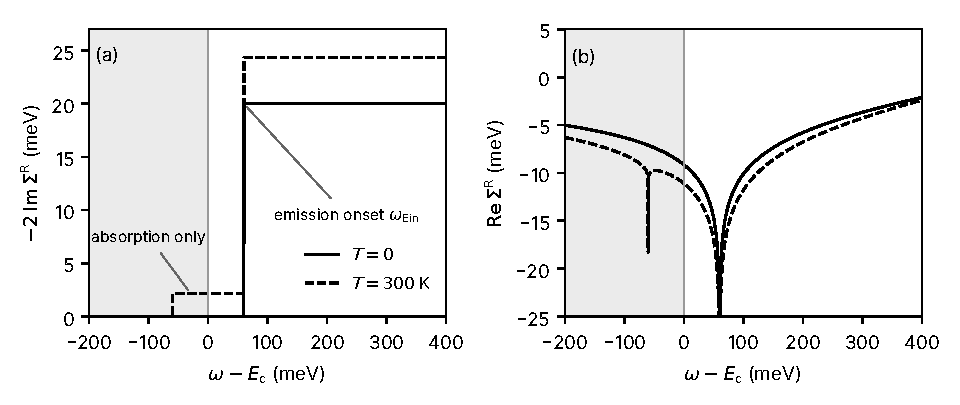
\includegraphics[width=\linewidth]{figures/ch04/fig4_9b.pdf}
  \caption{Self-energy of an electron coupled to a dispersionless boson of energy $\omega_{\mathrm{Ein}} = \SI{60}{meV}$ (\cref{we:4-einstein}), against the energy $\omega$ measured from the bottom $E_{\mathrm{c}}$ of an empty band with a flat density of states over $E_{\mathrm{w}} = \SI{1}{eV}$, for a constant coupling with the golden-rule emission rate $\varGamma_{\mathrm{em}} = \SI{20}{meV}$; solid at $T = 0$, dashed at \SI{300}{K}. The model and its parameters are illustrative. (a) The width $-2\Imag\Sigma^{\mathrm{R}}$: zero below the emission threshold $E_{\mathrm{c}} + \omega_{\mathrm{Ein}}$ at $T = 0$; at \SI{300}{K}, $\varGamma_{\mathrm{em}}n_{\mathrm{B}} = \SI{2.2}{meV}$ from absorption above $E_{\mathrm{c}} - \omega_{\mathrm{Ein}}$, and $\varGamma_{\mathrm{em}}(2n_{\mathrm{B}} + 1)$ where both processes are allowed. (b) The shift $\Real\Sigma^{\mathrm{R}}$, $\SI{-9.14}{meV}$ at $E_{\mathrm{c}}$ for $T = 0$ and $\SI{-11.09}{meV}$ at \SI{300}{K}, with logarithmic singularities at the thresholds caused by the sharp edge of the flat band. Shaded: below the band bottom.}
  \label{fig:4-einstein}
\end{figure}

\subsection{The screened interaction and the \texorpdfstring{$GW$}{GW} self-energy}

The Coulomb version of the same diagram, with a bare line, is the exchange self-energy \cref{eq:D.11-fock}, $\Sigma_{\mathrm{x}}(\vect{k}) = -\Vol^{-1}\sum_{\vect{p}}v_{\mathrm{C}}(|\vect{k} - \vect{p}|)\,n_{\mathrm{F}}(\xi_{\vect{p}})$, the Fock term. It is static, it has no imaginary part, and in a metal it makes the group velocity of the electron gas infinite at the Fermi surface through a logarithm (\cref{app:D.4}). What it misses is screening: while the electron propagates, the other electrons rearrange around it and weaken the interaction at long distances. The rules say how to put this in. Every chain of bubbles that can be inserted into the Coulomb line is a self-energy diagram, and summing the chains replaces the line, exactly as in the random-phase chain:
\begin{equation}
  W^{\mathrm{scr}}(\vect{q},\ii\omega^{\mathrm{B}}_j) = v_{\mathrm{C}}(q) + v_{\mathrm{C}}(q)\,R(\vect{q},\ii\omega^{\mathrm{B}}_j)\,v_{\mathrm{C}}(q) = \varepsilon^{-1}(\vect{q},\ii\omega^{\mathrm{B}}_j)\,v_{\mathrm{C}}(q) .
  \label{eq:4.8-W}
\end{equation}
The last step is \cref{eq:4.4-eps}. With the bubble chain alone, $R$ is the random-phase response \cref{eq:4.8-chain} and $\varepsilon$ the Lindhard function of \cref{sec:4.5} or its crystal form; with the proper blobs it is exact. The screened interaction is the Coulomb potential of a test charge seen through the dielectric response of the target, the same $\varepsilon^{-1}v_{\mathrm{C}}$ that \cref{sec:4.4} found for an external charge, but now at every frequency. In a crystal it is the matrix $W^{\mathrm{scr}}_{\vect{G}\vect{G}'} = (\varepsilon^{-1})_{\vect{G}\vect{G}'}v_{\mathrm{C}}(|\vect{q}+\vect{G}'|)$, and the steps below hold element by element.

Replacing the bare line of the exchange diagram by $W^{\mathrm{scr}}$, and the free propagator by the full one, is the $GW$ approximation of Hedin~\cite{hedin1965new}. In imaginary time,
\begin{equation}
  \Sigma(\vect{k},\ii\omega^{\mathrm{F}}_j) = -\frac1\Vol\sum_{\vect{q}}T\sum_{j'}W^{\mathrm{scr}}(\vect{q},\ii\omega^{\mathrm{B}}_{j'})\,\GF(\vect{k} - \vect{q},\ii\omega^{\mathrm{F}}_j - \ii\omega^{\mathrm{B}}_{j'}) ,
  \label{eq:4.8-GWmats}
\end{equation}
with the convergence factor of rule 5 on the static part $v_{\mathrm{C}}$, which reproduces $\Sigma_{\mathrm{x}}$. At $T = 0$ the real-time rules give the same diagram as
\begin{equation}
  \Sigma(\vect{k},\omega) = \frac{\ii}{\Vol}\sum_{\vect{q}}\int\frac{\dd\omega'}{2\pi}\,\GF(\vect{k} - \vect{q},\omega - \omega')\,W^{\mathrm{scr}}(\vect{q},\omega') ,
  \label{eq:4.8-GW}
\end{equation}
which in space and time is a product, $\Sigma(1,2) = \ii\GF(1,2)W^{\mathrm{scr}}(1,2)$, the form usually written $\Sigma = \ii GW$~\cite[Eqs.~(60) and (61)]{aryasetiawan1998gw}. Note that $\GF$ and $W^{\mathrm{scr}}$ here are time-ordered functions: by the convention of \cref{sec:4.7}, a function without superscript and with a real argument is time-ordered, and $W^{\mathrm{scr}}(\vect{q},\omega')$ equals the retarded $\varepsilon^{-1}v_{\mathrm{C}}$ of \cref{sec:4.4} for $\omega' > 0$ and the advanced one for $\omega' < 0$. Lifetimes need the retarded self-energy, which the Matsubara form \cref{eq:4.8-GWmats} delivers by continuation. The approximation keeps the screening to all orders and drops the vertex corrections, the diagrams in which a further line crosses the one of \cref{fig:4-diagrams}c; Hedin's exact equations contain them in a vertex function, which the $GW$ approximation sets to one~\cite[Eqs.~(43)--(46)]{aryasetiawan1998gw}. With the Hartree term, which is the electrostatic potential of the density, $GW$ is the self-energy behind the quasiparticle gap of silicon in \cref{sec:3.4,sec:4.7}.

The lifetime follows from the same frequency sum as for a boson. The difference $W^{\mathrm{scr}} - v_{\mathrm{C}} = v_{\mathrm{C}}^2R$ is a response function, and like every response it has the spectral representation \cref{eq:4.2-spectral}, $W^{\mathrm{scr}}(\vect{q},z) - v_{\mathrm{C}}(q) = \int\dd\omega'\,B(\vect{q},\omega')/(z - \omega')$, with the weight $B = -\Imag W^{\mathrm{scr},\mathrm{R}}/\pi = v_{\mathrm{C}}(q)L(\vect{q},\omega')/\pi$, where $L$ is the loss function \cref{eq:4.4-SL}. This is a superposition of bosons: the free boson line has $B = |g|^2[\delta(\omega' - \omega_{\vect{Q}}) - \delta(\omega' + \omega_{\vect{Q}})]$, and the screened Coulomb line is a continuum of them, the electron--hole pairs and plasmons of the target, weighted by the loss function. The residue sum that led to \cref{eq:4.8-sigmaboson} then leads, with the free propagator in \cref{eq:4.8-GWmats},
\begin{equation*}
  \Sigma(\vect{k},\ii\omega^{\mathrm{F}}_j) = \Sigma_{\mathrm{x}}(\vect{k}) + \frac1\Vol\sum_{\vect{q}}\int\dd\omega'\,B(\vect{q},\omega')\,\frac{n_{\mathrm{B}}(\omega') + 1 - n_{\mathrm{F}}(\xi_{\vect{k}-\vect{q}})}{\ii\omega^{\mathrm{F}}_j - \xi_{\vect{k}-\vect{q}} - \omega'} ,
\end{equation*}
and the imaginary part of its continuation, $\Imag\Sigma^{\mathrm{R}}(\vect{k},\omega) = -\Vol^{-1}\sum_{\vect{q}}v_{\mathrm{C}}(q)L(\vect{q},\omega')[n_{\mathrm{B}}(\omega') + 1 - n_{\mathrm{F}}(\xi_{\vect{k}-\vect{q}})]$ with $\omega' = \omega - \xi_{\vect{k}-\vect{q}}$. On the shell $\omega = \xi_{\vect{k}}$, with $z_{\mathrm{qp}} \simeq 1$, the width is $\varGamma_{\mathrm{qp}} = -2\Imag\Sigma^{\mathrm{R}}$. The structure-factor relation $2L/v_{\mathrm{C}} = (1 - \ee^{-\beta\omega'})S$ of \cref{eq:4.4-SL}, and the identity $(1 - \ee^{-\beta\omega'})(n_{\mathrm{B}}(\omega') + 1) = 1$, turn it into a rate.
\begin{keyresult}[Electron--electron lifetime in the $GW$ approximation]
\begin{equation}
  \varGamma_{\mathrm{qp}}(\vect{k}) = \int\frac{\dd^3q}{(2\pi)^3}\,v_{\mathrm{C}}(q)^2\,S(\vect{q},\omega')\Bigl[1 - n_{\mathrm{F}}(\xi_{\vect{k}-\vect{q}}) + \ee^{-\beta\omega'}n_{\mathrm{F}}(\xi_{\vect{k}-\vect{q}})\Bigr], \qquad \omega' = \xi_{\vect{k}} - \xi_{\vect{k}-\vect{q}} .
  \label{eq:4.8-lifetime}
\end{equation}
The inverse lifetime of an electron is the rate \cref{eq:4.2-rate} at which it would scatter off the target as a projectile with the potential $\tilde V = v_{\mathrm{C}}$, with the Pauli factor of its final state, plus the rate of the reverse process.
\end{keyresult}
An injected electron is thus a dark-matter particle with a Coulomb coupling. It loses energy to exactly the excitations that the loss function describes, through the same structure factor, and \cref{eq:4.8-lifetime} is a stopping-power calculation of the kind in \cref{eq:4.4-dEdx}, with a quantum recoil and a Pauli-blocked final state. The reverse term, $\ee^{-\beta\omega'}n_{\mathrm{F}}$, is the rate at which electrons in $\vect{k} - \vect{q}$ absorb energy from the target and refill $\vect{k}$, and it is negligible for an electron far above $\mu_{\mathrm{ch}}$. Near the Fermi level of a metal, $1 - n_{\mathrm{F}}$ and the linear low-frequency loss function of \cref{sec:4.5} give the $\xi_{\vect{k}}^2$ of \cref{sec:4.7}. In silicon, $S(\vect{q},\omega')$ vanishes for $\omega'$ below the gap, and an electron cannot decay by creating a pair until it sits at least $\Eg$ above the band edge. Higher up, the loss function peaks at the plasmon near \SI{16.4}{eV} (\cref{sec:4.4}), and an electron with tens of eV loses its energy mostly by plasmon emission. The exchange of the projectile with the electrons it excites, a vertex correction, is absent from \cref{eq:4.8-lifetime}.

In practice the $GW$ quasiparticle energies and lifetimes of silicon are computed in the basis of Kohn--Sham states. The independent-electron response $R^0_{\vect{G}\vect{G}'}$ of \cref{sec:4.6} yields $\varepsilon^{-1}_{\vect{G}\vect{G}'}$ in the random-phase approximation, and \cref{eq:4.8-W} gives the matrix $W^{\mathrm{scr}}_{\vect{G}\vect{G}'}$. The matrix elements $\langle\psi_{n\vect{k}}|\Sigma(\omega)|\psi_{n\vect{k}}\rangle$ of \cref{eq:4.8-GW}, built from the same plane-wave matrix elements, enter the linearized quasiparticle equation \cref{eq:4.7-G0W0}. The frequency integral is the expensive step: a plasmon-pole model, which puts each element of $\Imag\varepsilon^{-1}$ into a single delta function, is accurate for the energies; however, it produces no lifetimes, which need $\Imag\varepsilon^{-1}$ resolved down to the gap.

\subsection{The cutting rule}

The imaginary parts found so far have all been golden-rule rates: the transition sums in \cref{eq:4.7-bubble}, the emission and absorption rates of \cref{we:4-einstein}, the scattering rate \cref{eq:4.8-lifetime}. This is general, and it has a graphical form. After the frequency sums, a diagram at real frequency is a sum of terms, each a product of occupation factors divided by $\omega - E_{\mathrm{cs}} + \ii0^+$, where $E_{\mathrm{cs}}$ is the total energy of a set of lines that together separate the two external points. Its imaginary part replaces each such denominator by $-\pi\delta(\omega - E_{\mathrm{cs}})$, by the Sokhotski--Plemelj formula \cref{eq:2.4-SP}. Drawing a line through the diagram across these propagators, the cut, puts them on shell. The pieces on either side of the cut are the amplitudes to reach the cut state and to return from it, and the imaginary part is $\pi$ times their product summed over the cut states: a golden-rule rate. Cutkosky formulated this rule for relativistic amplitudes~\cite{cutkosky1960singularities}. At finite temperature the occupation factors combine into rates in two ways, and Weldon gave the general form~\cite{weldon1983simple}; we show it for the two diagrams that the book uses.

For the boson self-energy \cref{eq:4.8-sigmaboson}, the cut runs through the electron line and the boson line. Write each thermal factor on its shell as a sum of products of occupations, $n_{\mathrm{B}} + 1 - n_{\mathrm{F}} = (1 + n_{\mathrm{B}})(1 - n_{\mathrm{F}}) + n_{\mathrm{B}}n_{\mathrm{F}}$ and $n_{\mathrm{B}} + n_{\mathrm{F}} = n_{\mathrm{B}}(1 - n_{\mathrm{F}}) + (1 + n_{\mathrm{B}})n_{\mathrm{F}}$. With $\xi' = \xi_{\vect{k}-\vect{Q}}$ and $n_{\mathrm{F}} = n_{\mathrm{F}}(\xi')$,
\begin{equation}
  \begin{gathered}
  -2\Imag\Sigma^{\mathrm{R}}(\vect{k},\omega) = \varGamma_{\mathrm{out}}(\vect{k},\omega) + \varGamma_{\mathrm{in}}(\vect{k},\omega), \\
  \varGamma_{\mathrm{out}} = \frac{2\pi}{\Vol}\sum_{\vect{Q}}|g(\vect{Q})|^2(1 - n_{\mathrm{F}})\Bigl[(1 + n_{\mathrm{B}})\,\delta(\omega - \xi' - \omega_{\vect{Q}}) + n_{\mathrm{B}}\,\delta(\omega - \xi' + \omega_{\vect{Q}})\Bigr], \\
  \varGamma_{\mathrm{in}} = \frac{2\pi}{\Vol}\sum_{\vect{Q}}|g(\vect{Q})|^2\,n_{\mathrm{F}}\Bigl[n_{\mathrm{B}}\,\delta(\omega - \xi' - \omega_{\vect{Q}}) + (1 + n_{\mathrm{B}})\,\delta(\omega - \xi' + \omega_{\vect{Q}})\Bigr] .
  \end{gathered}
  \label{eq:4.8-cutsigma}
\end{equation}
$\varGamma_{\mathrm{out}}$ is the golden-rule rate \cref{eq:2.1-golden} at which an electron in $\vect{k}$ with energy $\omega$ scatters out, by emission or absorption, into an empty state. $\varGamma_{\mathrm{in}}$ is the rate at which electrons scatter into an empty $\vect{k}$ from occupied states. On the shell, $n_{\mathrm{B}}/(1 + n_{\mathrm{B}}) = \ee^{-\beta\omega_{\vect{Q}}}$ and $n_{\mathrm{F}}/(1 - n_{\mathrm{F}}) = \ee^{-\beta\xi'}$, so that $\varGamma_{\mathrm{in}} = \ee^{-\beta\omega}\varGamma_{\mathrm{out}}$, the fermion counterpart of detailed balance. The retarded Green's function is built from an anticommutator, and its width counts the decay of an added electron and the filling of an added hole together. The density response is built from a commutator, and the corresponding combination is a difference.
\begin{keyresult}[Cutting rule]
The imaginary part of the retarded continuation of a diagram is the sum over its cuts, each cut line on shell. For a fermion self-energy, $-2\Imag\Sigma^{\mathrm{R}} = \varGamma_{\mathrm{out}}(1 + \ee^{-\beta\omega})$ with $\varGamma_{\mathrm{out}}$ the golden-rule rate out of the state; for a density response, $-2\Imag R = (1 - \ee^{-\beta\omega})S$ with $S$ the golden-rule sum into the cut states.
\end{keyresult}

\begin{workedexample}{The cut of the bubble}\label{we:4-cut}
The bubble has a single cut, through its two propagators (\cref{fig:4-cut}), and its cut state is one electron--hole pair. With orbitals $\gamma$ in place of plane waves, the density vertex between $\gamma$ and $\gamma'$ is $\langle\gamma'|\ee^{\ii\vect{q}\cdot\vect{r}}|\gamma\rangle$, and the frequency sum \cref{eq:D.10-sum} gives
\begin{equation*}
  R^0(\vect{q},\ii\omega^{\mathrm{B}}_j) = \frac1\Vol\sum_{\gamma\gamma'}\bigl|\langle\gamma'|\ee^{\ii\vect{q}\cdot\vect{r}}|\gamma\rangle\bigr|^2\,\frac{n_\gamma - n_{\gamma'}}{\ii\omega^{\mathrm{B}}_j + E_\gamma - E_{\gamma'}} ,
\end{equation*}
with $n_\gamma = n_{\mathrm{F}}(E_\gamma - \mu_{\mathrm{ch}})$; for plane waves the matrix element is $\delta_{\vect{k}',\vect{k}+\vect{q}}$ and this is \cref{eq:4.7-bubble}. The denominator is $\omega - E_{\mathrm{cs}}$ with $E_{\mathrm{cs}} = E_{\gamma'} - E_\gamma$, the energy of the pair. Continuing to $\omega + \ii0^+$ and cutting,
\begin{equation*}
  -2\Imag R^0(\vect{q},\omega) = \frac{2\pi}{\Vol}\sum_{\gamma\gamma'}\bigl|\langle\gamma'|\ee^{\ii\vect{q}\cdot\vect{r}}|\gamma\rangle\bigr|^2\,(n_\gamma - n_{\gamma'})\,\delta(\omega - E_{\gamma'} + E_\gamma) .
\end{equation*}
The Pauli difference is a difference of two rates. On the shell, $n_{\gamma'}(1 - n_\gamma) = \ee^{-\beta\omega}n_\gamma(1 - n_{\gamma'})$, and $n_\gamma - n_{\gamma'} = n_\gamma(1 - n_{\gamma'}) - n_{\gamma'}(1 - n_\gamma) = (1 - \ee^{-\beta\omega})\,n_\gamma(1 - n_{\gamma'})$: an electron moves from occupied $\gamma$ to empty $\gamma'$, minus the reverse move. The factor $1 - \ee^{-\beta\omega}$ is that of the fluctuation--dissipation theorem \cref{eq:4.2-fdt}, and what it multiplies is
\begin{equation*}
  S^0(\vect{q},\omega) = \frac{2\pi}{\Vol}\sum_{\gamma\gamma'}\bigl|\langle\gamma'|\ee^{\ii\vect{q}\cdot\vect{r}}|\gamma\rangle\bigr|^2\,n_\gamma(1 - n_{\gamma'})\,\delta(\omega - E_{\gamma'} + E_\gamma) ,
\end{equation*}
the golden-rule sum \cref{eq:4.2-S0} over single electron--hole pairs, term by term; for the electron gas at $T = 0$ it is the closed form \cref{eq:4.2-gas}. The terms with $\gamma' = \gamma$ have $n_\gamma - n_{\gamma'} = 0$ and drop out of the bubble; they are the elastic term of \cref{eq:4.2-S0}, which carries no dissipation.
\end{workedexample}

\begin{figure}[tbp]
  \centering
  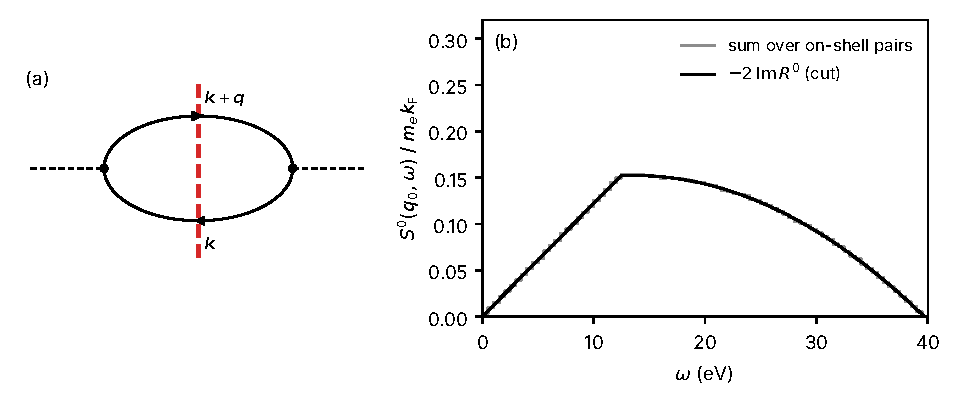
\includegraphics[width=0.45\linewidth]{figures/ch04/fig4_10.pdf}
  \caption{The cut of the bubble. The dashed stubs mark the external momentum $\vect{q}$ at the two density vertices. The cut (dashed vertical line) passes through the electron line $\vect{k}+\vect{q}$ and the hole line $\vect{k}$ and puts both on shell, $\omega = \xi_{\vect{k}+\vect{q}} - \xi_{\vect{k}}$; each half of the diagram is the amplitude for the density operator to create the pair.}
  \label{fig:4-cut}
\end{figure}

Whatever diagram is drawn, its imaginary part counts real final states with positive weights, and every approximation that is a selection of diagrams, with the cuts it allows, has a golden-rule reading. The random-phase chain cuts through electron--hole pairs and plasmons. The ladder, which \cref{sec:4.9} sums, cuts through pairs whose electron and hole are bound into excitons.
